\documentclass{article}

\usepackage{graphicx}
\usepackage{tikz}
\usepackage{tikzsymbols}
\usetikzlibrary{calc,patterns,shapes.geometric}
\pagestyle{empty}
\usepackage[margin=0pt]{geometry}
\geometry{papersize={14in,12in}}

\def\centerarc[#1](#2)(#3:#4:#5){\draw[#1] ($(#2)+({#5*cos(#3)},{#5*sin(#3)})$) arc (#3:#4:#5);}

\begin{document}
	\begin{figure}
		\centering
		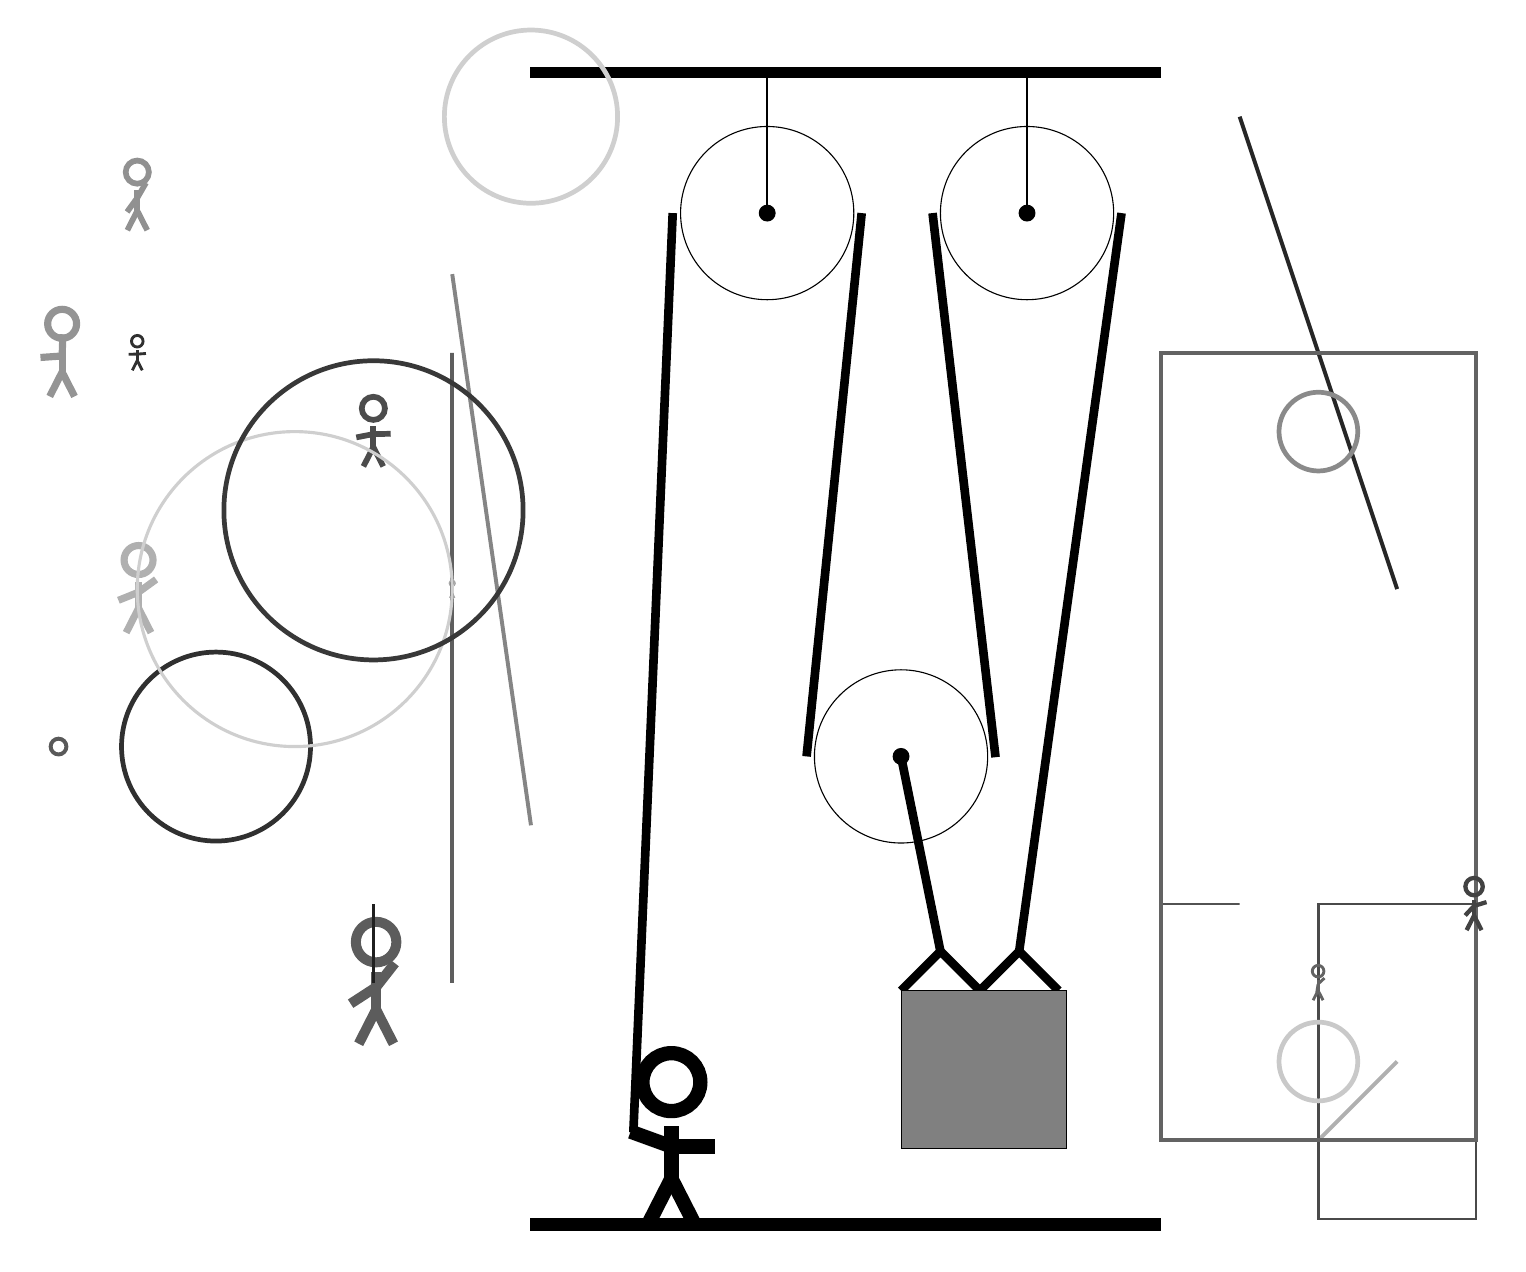
\begin{tikzpicture}
			%%%%% START %%%%%
			
			\draw[fill=black] (-2, 11.5) rectangle (6, 11.625);
			
			\draw (1, 9.775) circle (1.1);
			\draw[fill=black] (1, 9.775) circle (0.1);
			\draw[thick] (1, 9.775) -- (1, 11.5);
			
			\draw (4.3, 9.775) circle (1.1);
			\draw[fill=black] (4.3, 9.775) circle (0.1);
			\draw[thick] (4.3, 9.775) -- (4.3, 11.5);
			
			\draw (2.7, 2.875) circle (1.1);
			\draw[fill=black] (2.7, 2.875) circle (0.1);
			
			\draw[line width=1.1mm]  (2.7, -0.1) -- (3.2, 0.4) -- (3.7, -0.1) -- (4.2, 0.4) -- (4.7, -0.1);
			\draw[fill=black!50] (2.7, -0.1) rectangle (4.8, -2.1);
			
			\node[line width=0.3mm, color=black!70] at (-4, 7) {\Strichmaxerl[4][11][1]};
			
			\draw[line width=0.5mm, color=black!31](8, -2) -- (9, -1);
			\node[line width=0.3mm, color=black!35] at (-3, 5) {\Strichmaxerl[1][82][89]};
			\draw[line width=0.2mm, color=black!68] (6, 1) rectangle (7, 1);
			
			\node[line width=0.2mm, color=black!64] at (-4, 0) {\Strichmaxerl[7][33][52]};
			\draw[line width=0.3mm, color=black!71] (8, 1) rectangle (10, -3);
			\draw[line width=0.5mm, color=black!85](7, 11) -- (9, 5);
			\draw [line width=0.6mm, color=black!81](-6, 3) circle (1.2);
			\draw[line width=0.4mm, color=black!88] (-4, 0) rectangle (-4, 1);
			
			\draw[line width=0.5mm, color=black!63] (-3, 0) rectangle (-3, 8);
			\node[line width=0.3mm, color=black!42] at (-8, 8) {\Strichmaxerl[5][4][88]};
			\draw [line width=0.6mm, color=black!19](-2, 11) circle (1.1);
			\draw [line width=0.6mm, color=black!46](8, 7) circle (0.5);
			
			\node[line width=0.7mm, color=black!43] at (-7, 10) {\Strichmaxerl[4][54][60]};
			\node[line width=0.7mm, color=black!31] at (-7, 5) {\Strichmaxerl[5][22][36]};
			\draw [line width=0.4mm, color=black!19](-5, 5) circle (2.0);
			
			\draw[line width=0.5mm, color=black!61] (6, 8) rectangle (10, -2);
			\draw [line width=0.6mm, color=black!21](8, -1) circle (0.5);
			\node[line width=0.3mm, color=black!74] at (10, 1) {\Strichmaxerl[3][47][17]};
			
			\node[line width=0.4mm, color=black!61] at (8, 0) {\Strichmaxerl[2][81][43]};
			\draw [line width=0.5mm, color=black!65](-8, 3) circle (0.1);
			\node[line width=0.4mm, color=black!81] at (-7, 8) {\Strichmaxerl[2][1][4]};
			
			\draw[line width=0.5mm, color=black!48](-3, 9) -- (-2, 2);
			\draw [line width=0.6mm, color=black!78](-4, 6) circle (1.9);
			
			\draw[line width=1.1mm](-0.7, -1.9) -- (-0.2, 9.775);
			\centerarc[line width=1.1mm](1, 9.775)(0:180:1.2000000000000002);
			\draw[line width=1.1mm](2.2, 9.775) -- (1.5, 2.875);
			\centerarc[line width=1.1mm](2.7, 2.875)(180:370:1.2000000000000002);
			\draw[line width=1.1mm] (3.9, 2.865) -- (3.1, 9.775);
			\centerarc[line width=1.1mm](4.3, 9.775)(0:180:1.2000000000000002);
			\draw[line width=1.1mm](4.2, 0.4) -- (5.5, 9.775);
			\draw[line width=1.1mm] (3.2, 0.4) -- (2.7, 2.875);
			
			\node at (-0.2, -2) {\Strichmaxerl[10][-20][0]};
			
			\draw[fill=black] (-2, -3) rectangle (6, -3.15);
			
			%%%%% END %%%%%
		\end{tikzpicture}
	\end{figure}	
\end{document}